% ----------------------------------------------------------
% ARQUITETURA
% ----------------------------------------------------------
\section{Arquitetura}
Para o desenvolvimento do projeto, e tendo em vista que seria construída uma aplicação \textit{web} de página única, utilizamos de ferramentas que cerceiam o ecossistema de \ac{spa}. Para isso, dividimos o projeto em \textit{\gls{frontend}} e \textit{\gls{backend}} de modo que eles se comuniquem via protocolo \ac{http} com requisições e respostas no formato \ac{json}. Para o desenvolvimento do \textit{\gls{frontend}} utilizamos \textit{\gls{typescript}} por meio da biblioteca \gls{react}; o \textit{\gls{backend}} foi desenvolvido utilizando Java com o micro \textit{\gls{framework}} \textit{\gls{spring boot}}.

Em relação ao \textit{\gls{deploy}} das aplicações, o \textit{\gls{frontend}} está hospedado na plataforma \textit{\gls{netlify}}, que hospeda e mantém um site com implantação contínua e HTTPS, proporcionando uma melhor agilidade de desenvolvimento, enquanto o \textit{\gls{backend}} está hospedado no \gls{heroku}, que é uma plataforma como serviço de fácil manuseio e que permite a equipe ter um maior foco no desenvolvimento do projeto. Através do \gls{heroku} podemos também fazer a utilização do \gls{postgre} por meio do serviço de apoio \gls{heroku} Postgres.

Ademais, para o armazenamento de objetos como arquivos ou imagens, utilizamos a plataforma Cloudinary, principalmente por sua fácil integração com a linguagem de programação Java através de bibliotecas.

\subsection{Diagramas de arquitetura}
Os diagramas \autoref{fig-arq-app}, \autoref{fig-arq-tec} e \autoref{fig-arq-negocio} ilustram de modo geral a arquitetura planejada e implementada para a solução proposta, utilizando das tecnologias já citadas.

A \autoref{fig-arq-app} ilustra a aplicação construída seguindo o ecossistema \ac{spa}, onde o navegador carrega toda a aplicação hospedada no \textit{\gls{netlify}}, então realiza requisições para o \textit{\gls{backend}} hospedado no \gls{heroku}, recebendo respostas no formato \ac{json}, as quais são manipuladas e exibidas de acordo com a necessidade pelo \textit{TypeScript} da aplicação no navegador.

\begin{figure}[H]
	\centering
	\caption{\label{fig-arq-app}Arquitetura de Aplicação}
	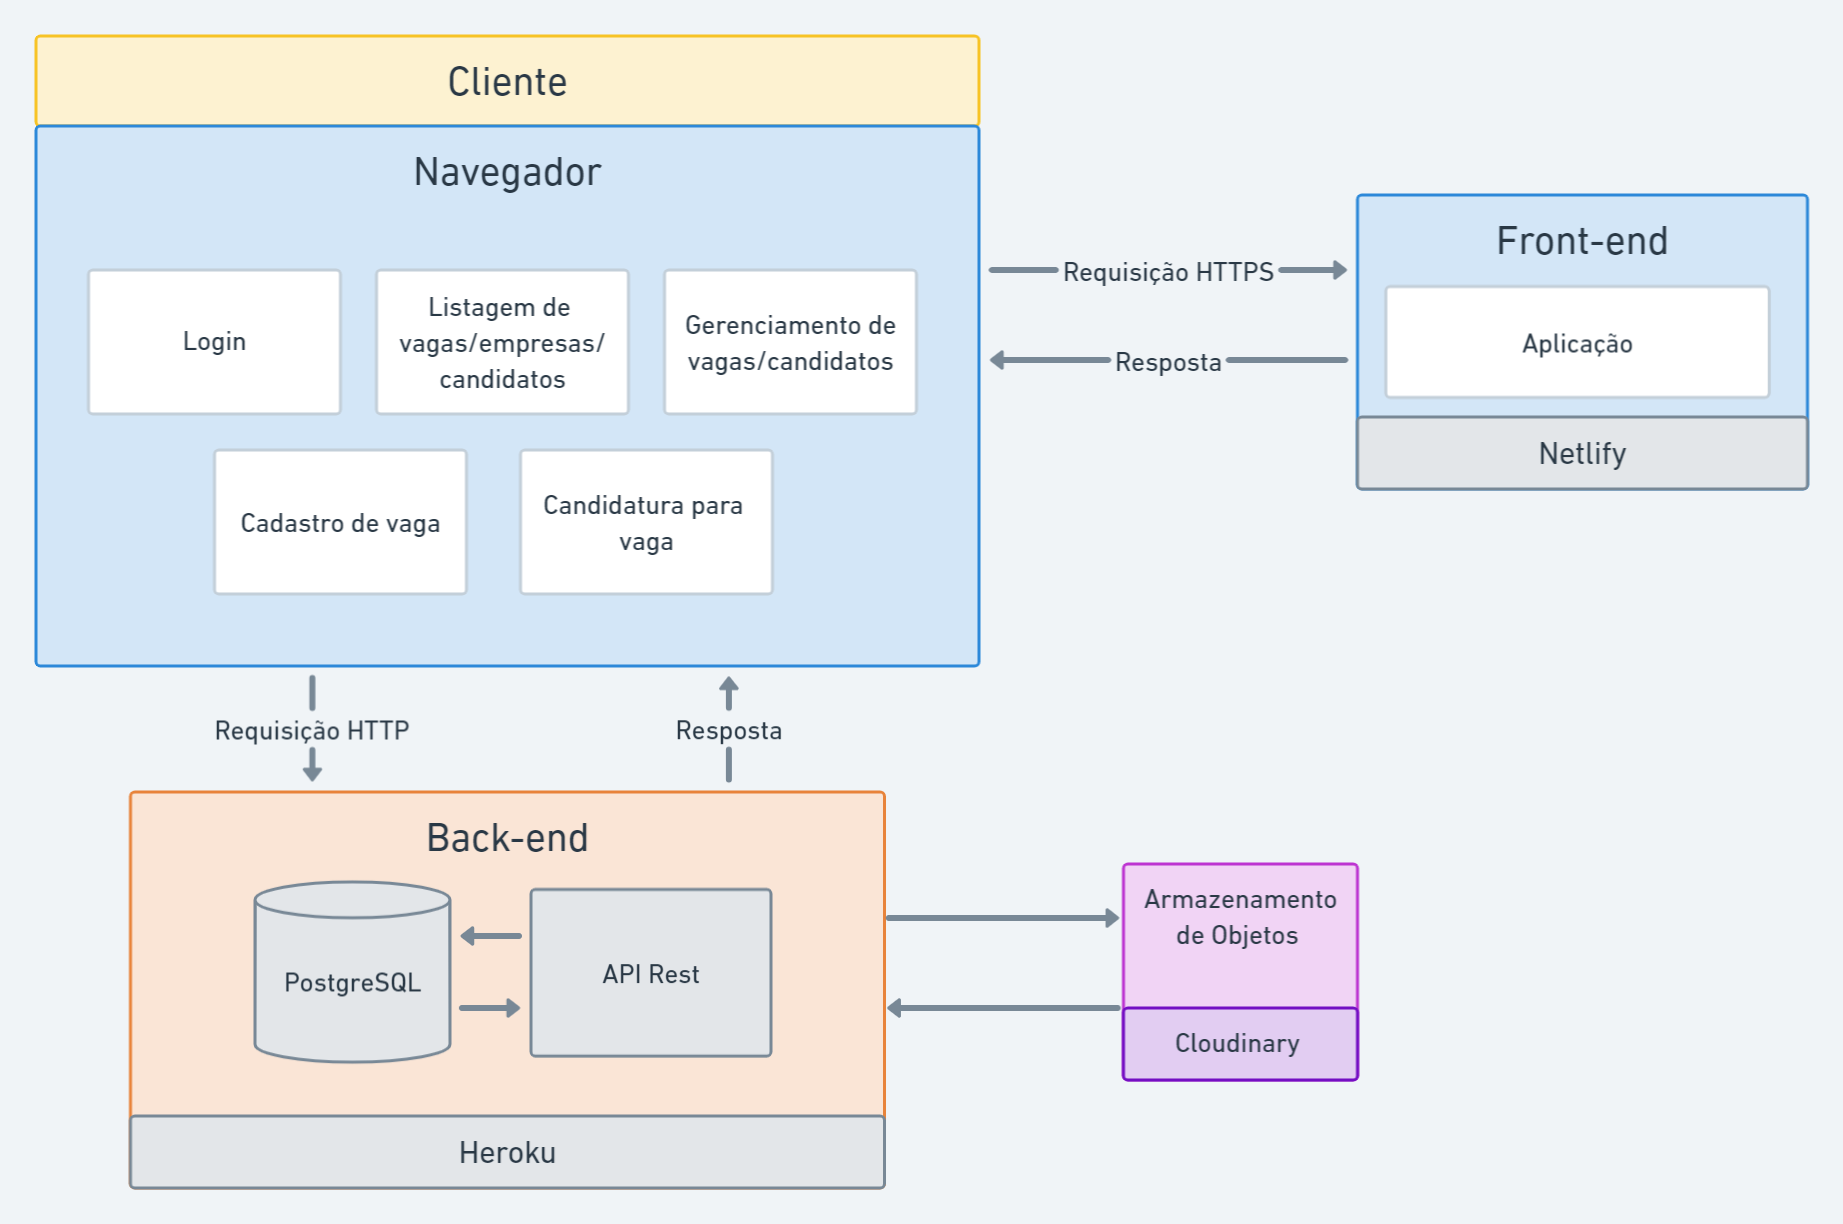
\includegraphics[width=0.95\textwidth]{../imagens/arq-proj-arq-app3.png}
	\fonte{Os Autores}
\end{figure}

A \autoref{fig-arq-tec} ilustra a mesma arquitetura, porém dando destaque para as tecnologias utilizadas tanto para hospedagem quanto desenvolvimento e versionamento.

\begin{figure}[H]
	\centering
	\caption{\label{fig-arq-tec}Arquitetura Tecnológica}
	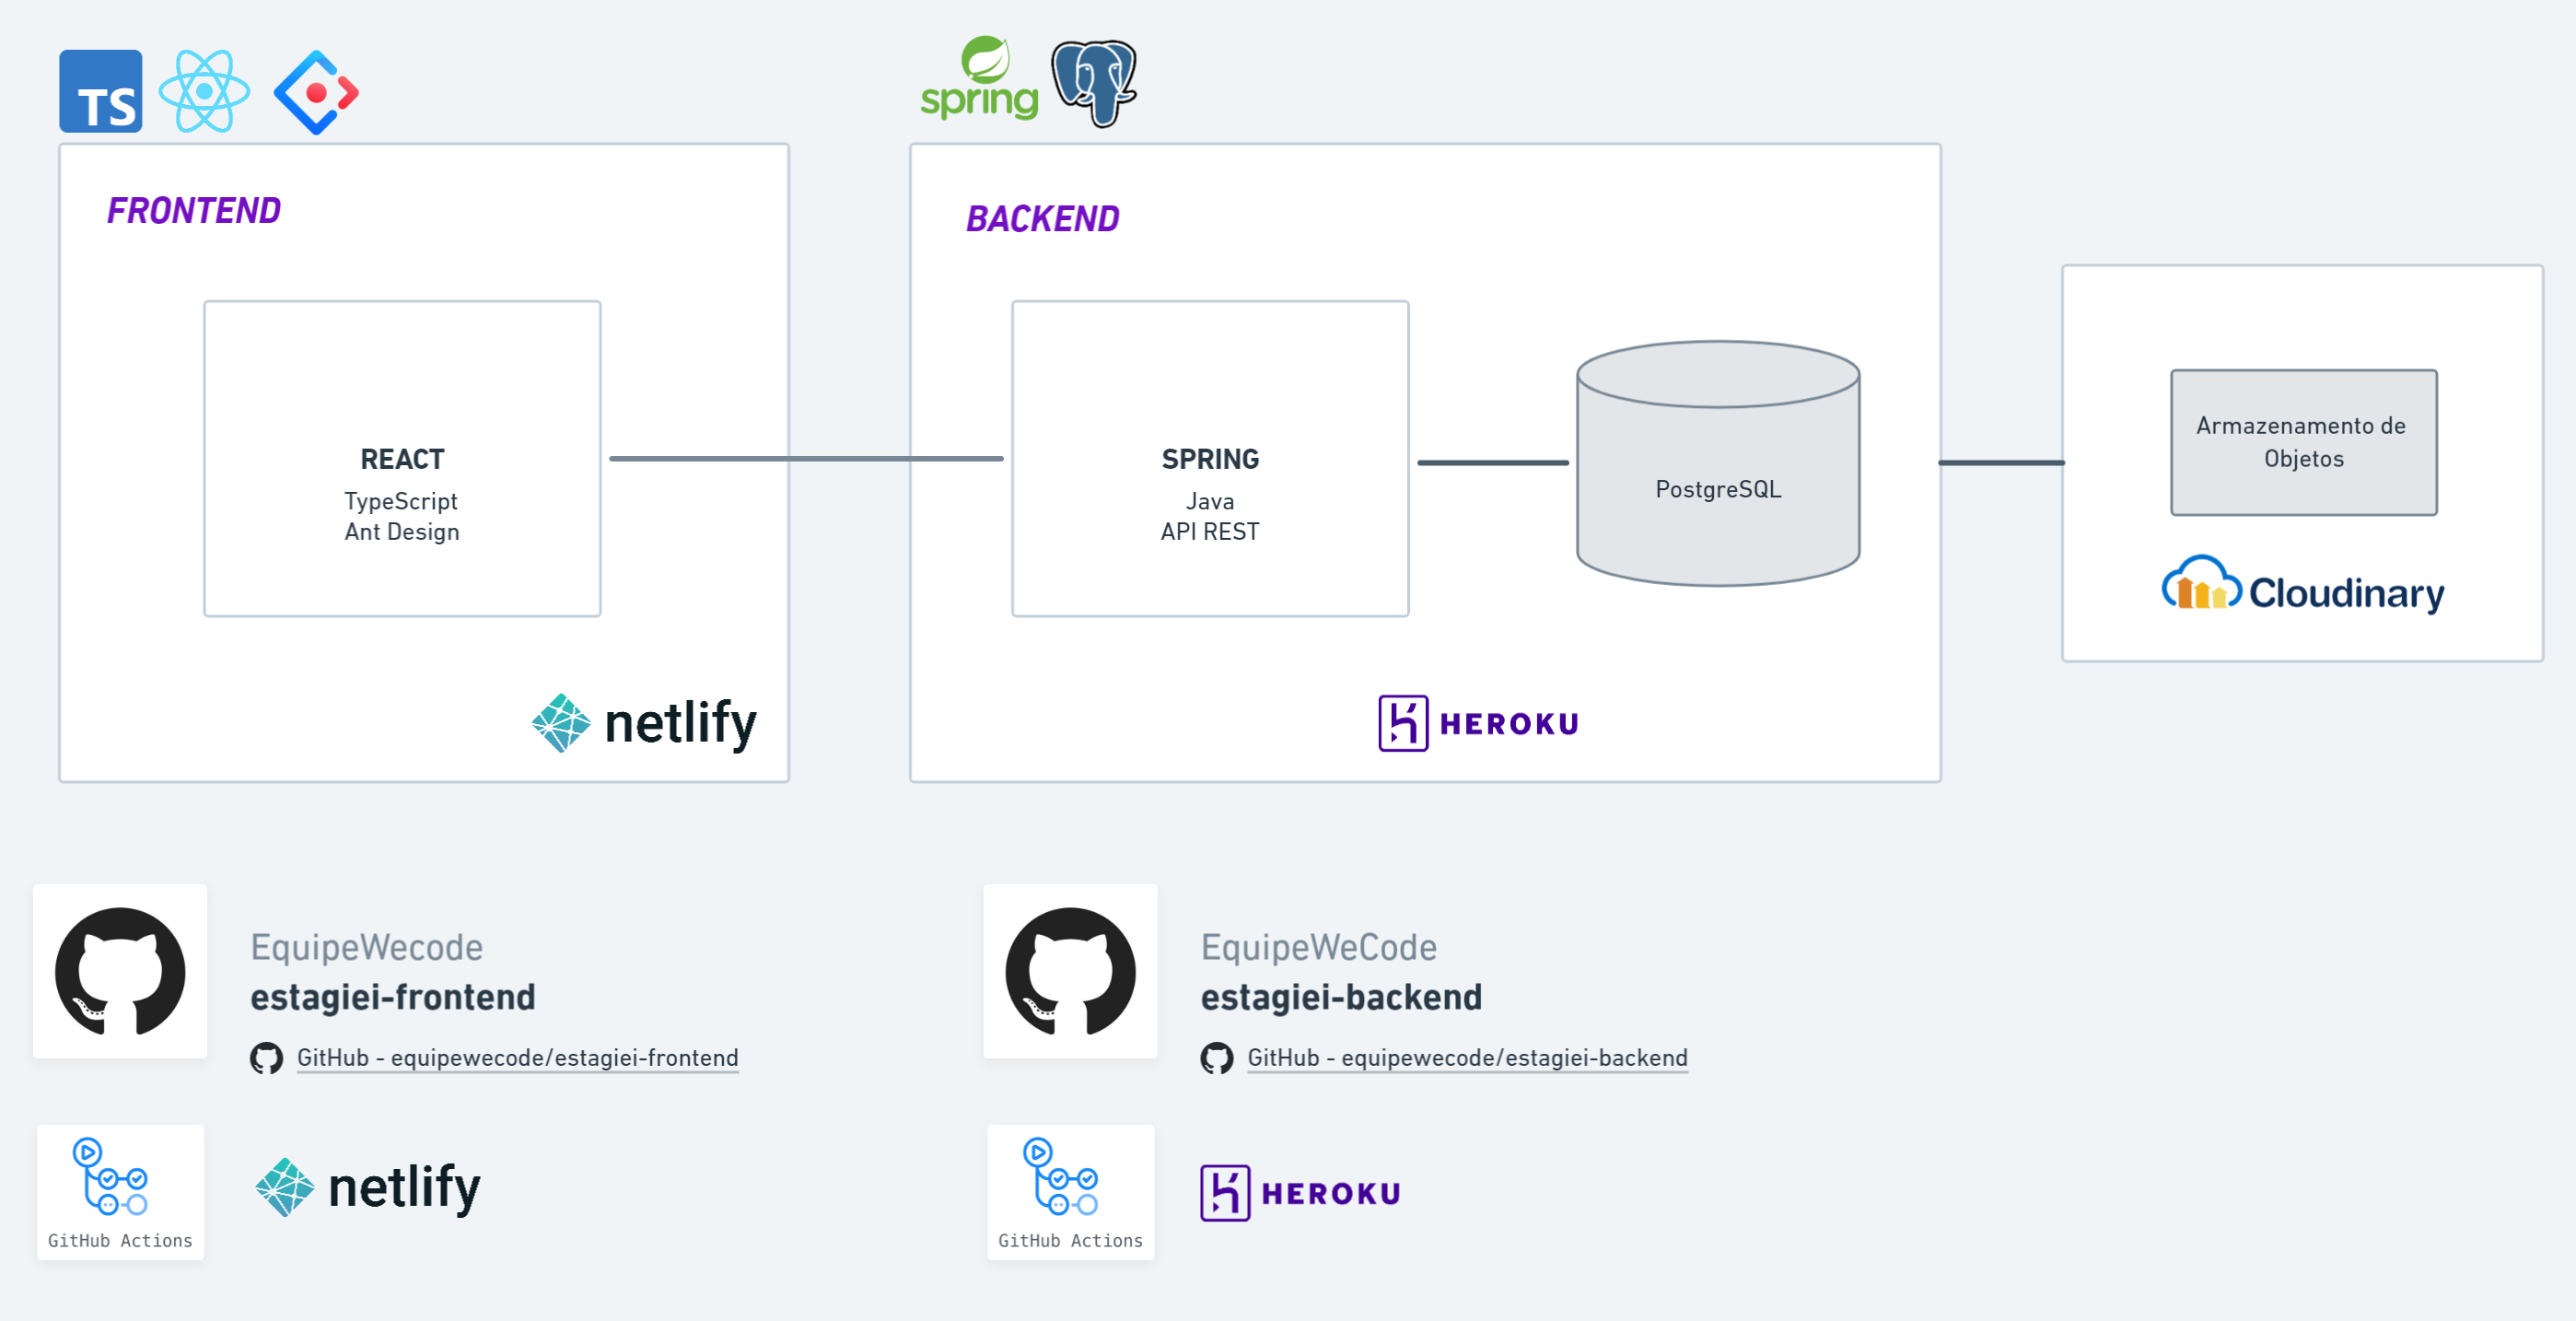
\includegraphics[width=0.95\textwidth]{../imagens/arq-proj-arq-tec4.png}
	\fonte{Os Autores}
\end{figure}

A \autoref{fig-arq-negocio} por sua vez, resume a ideia de negócio por trás do sistema \emph{EstagiEI} com relação ao cadastramento de empresas e estudantes (Candidato), suas ações com as vagas (cadastramento ou candidatura), o gerenciamentos de suas relações com as vagas e o recebimento de recomendações, sendo para empresa de candidatos e os estudantes recebem vagas de acordo com seu perfil.

\begin{figure}[H]
	\centering
	\caption{\label{fig-arq-negocio}Arquitetura de Negócios}
	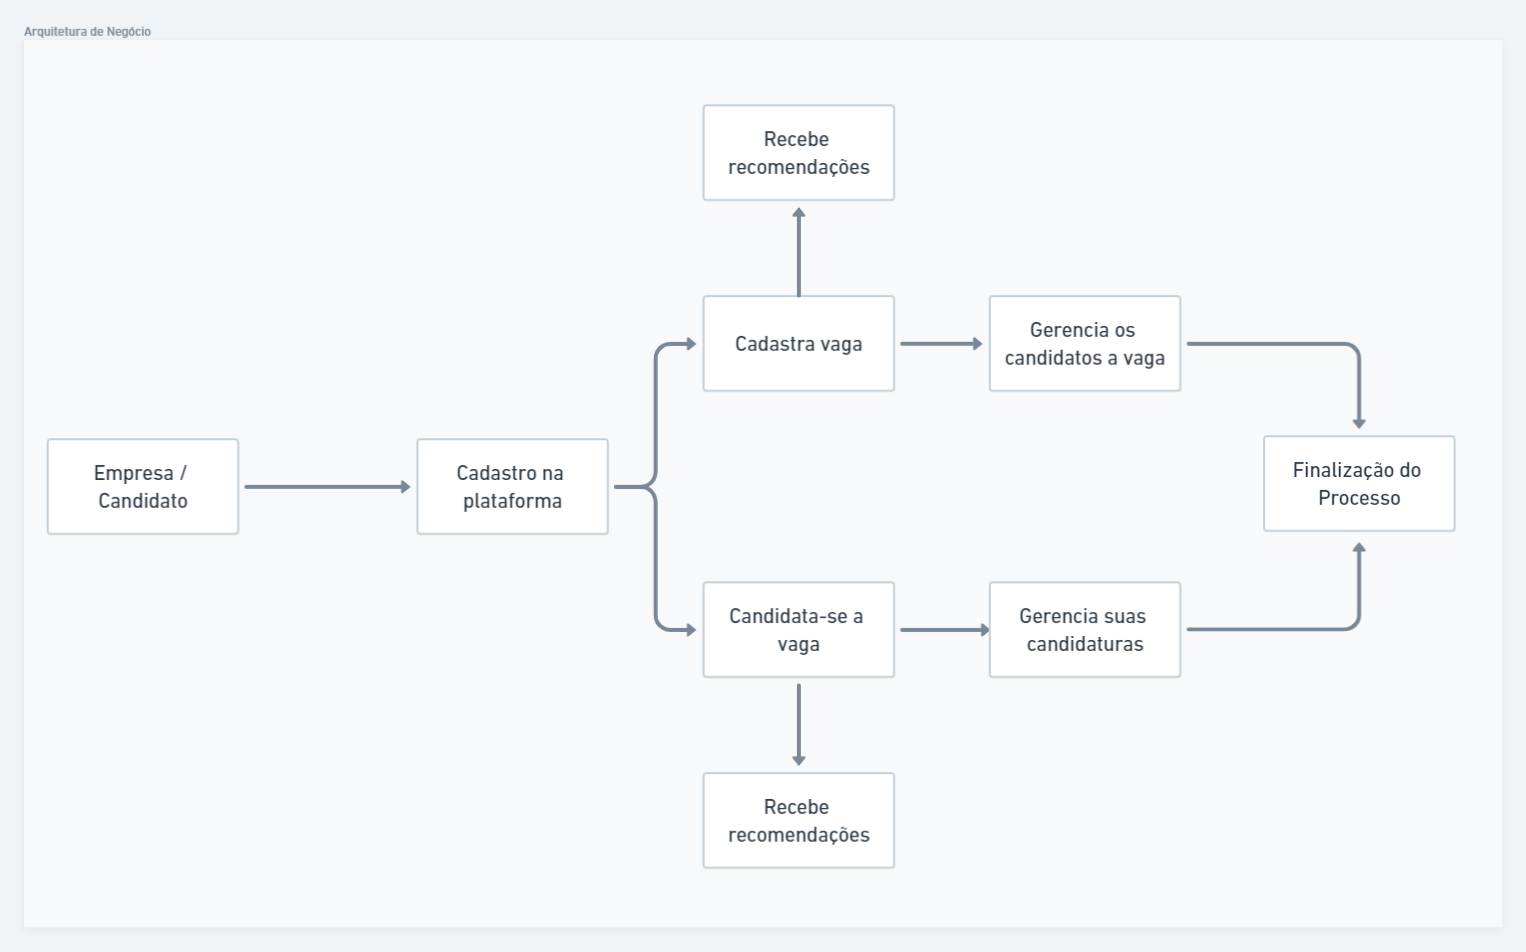
\includegraphics[width=0.95\textwidth]{../imagens/arq-proj-arq-negocio2.png}
	\fonte{Os Autores}
\end{figure}